\section{Background Theory}
In this section we present some of the relevant background theory from differential geometry that informs the primary topic and results of the project. This section is also a brief summary of the theory learned during the course of the project. The majority of the theory presented in this section can be found in \cite{andrews,burger2016riemannian,hitchin_2012,MR2954043}.
\subsection{Manifolds}
There are two primary (and equivalent) ways of characterising a smooth manifold. One way is by starting with a topological space and imposing further structure; the other is by starting with the concept of an abstract coordinate chart, building up to the notion of a differentiable structure and saying that a smooth manifold is simply a set with such a differentiable structure. In this report we will opt for the latter style of definition. As stated before, it can be shown that both definitions are in fact equivalent \cite{MR2954043,MR2766102}.\\

It should be noted that in the context of this project, we will always be working with \textit{smooth} manifolds and objects unless stated otherwise. By smooth it is meant, having derivatives of all orders. It is of course possible to develop the underlying theory discussed here without assuming smoothness but for this project we are interested in performing calculus and using analytical techniques on the objects of study and so proceed accordingly.
\begin{definition}
A \textit{coordinate chart} on a set $X$ is a subset $U\subseteq X$ together with a bijection, $$\varphi :U\to\varphi(U)\subseteq\mathbb{R}^n,$$ onto an open set $\varphi(U)$ in $\mathbb{R}^n$, denoted by $(U,\varphi)$.
\end{definition}
%One can then parametrise points $x$ of $U$ by $n$ coordinates given by $\varphi(x)=(x_1,\ldots,x_n)$.
\begin{definition}
A smooth $n$-dimensional \textit{atlas} on $X$ is a collection of coordinate charts $\left\{U_\alpha,\varphi_\alpha\right\}_{\alpha\in I}$ such that,
\begin{itemize}
\item $X$ is covered by the $\left\{U_\alpha\right\}_{\alpha\in I}$.
\item For each $\alpha,\beta\in I$, $\varphi_\alpha\left(U_\alpha\cap V_\alpha\right)$ is open in $\mathbb{R}^n$.
\item The map $$\varphi_\beta\circ\varphi_{\alpha}^{-1}:\varphi_\alpha\left(U_\alpha\cap U_\beta\right)\to\varphi_\beta\left(U_\alpha\cap U_\beta\right),$$ is a diffeomorphism (that is, the map is $C^{\infty}$ with a $C^{\infty}$ inverse).
\end{itemize}
\end{definition}
\begin{definition}
\label{def:atlas-compat}
Two atlases $\left\{\left(U_\alpha,\varphi_\alpha \right) \right\}$, $\left\{\left(V_i,\psi_i \right) \right\}$ are said to be \textit{compatible} if their union is an atlas.
\end{definition}
Definition \ref{def:atlas-compat} implies that the `extra' maps $\psi_i\varphi^{-1}_\alpha$ must all be smooth.
\begin{definition}
A \textit{differentiable structure} on $X$ is an equivalence class of atlases. Equivalently, one may say that a differentiable structure is given by a \textit{maximal} atlas on $X$. By maximal, we mean that given an atlas $\mathcal{A}$, there does not exist any atlas $\mathcal{B}$, such that $\mathcal{A}\subset \mathcal{B}$. 
\end{definition}
We may now define a smooth manifold as follows.
\begin{definition}
A $n$-dimensional \textit{differentiable (smooth) manifold} is a set $X$ equipped with a differentiable structure.
\end{definition}
As previously stated, there is an alternative characterisation of manifolds in which one starts with a topological space and imposes further structure on the space (e.g. requiring the space be Hausdorff, second countable, etc.). This would perhaps suggest that in order to prove facts about a manifold, one must first define a topology. However, we can show that the atlas gives us such a topology.\\

%\texttt{Needed?}
%Recall the definition of a topology.
%\begin{definition}
%Topology
%\end{definition}
Recall that a topology on a set $X$ is a collection of subsets of $X$ such that the collection is closed under arbitrary unions and finite intersections of elements in the subset. Elements of the topology are referred to as open sets.

We can define a topology on $M$ by saying that $U\subseteq W$ is open if and only for all $\alpha$, $\varphi_a(U\cap U_\alpha)$ is open in $\mathbb{R}^n$.

\begin{proposition}
Given the above topology, $\varphi_\alpha :U_\alpha\to\varphi_\alpha(U_\alpha)$ is a homeomorphism.
\end{proposition}
\begin{proof}
If $V\subseteq U_\alpha$ is open in the induced topology on $U_\alpha$, then since $U_\alpha$ is open, $V$ is open in $M$. By the definition of the topology, $\varphi_\alpha(V)=\varphi_\alpha(V\cap U_\alpha)$ is open. Hence, $\varphi^{-1}_\alpha$ is continuous.

Let $W\subset\varphi_\alpha(U_\alpha)$ be open. Then $\varphi_\alpha^{-1}(W)\subseteq U_\alpha$. We must prove that $\varphi_\alpha^{-1}(W)$ is open in $M$. We have,
\[
\varphi_\beta(\varphi_\alpha^{-1}(W)\cap U_\beta)=\varphi_\beta\varphi_\alpha^{-1}\left(W\cap\varphi_\alpha(U_\alpha\cap U_\beta)\right).
\]
From the definition of an atlas, the set $\varphi_\alpha(U_\alpha\cap U_\beta)$ is open. Thus, its intersection with the open set $W$ is open. Furthermore, $\varphi_\beta\circ\varphi_\alpha^{-1}$ is smooth with a smooth inverse, and so is certainly a homeomorphism. It follows that the right hand side of the above expression is open. Hence, $\varphi_\beta(\varphi_\alpha^{-1}(W)\cap U_\beta)$ is open and by definition of the topology, implies that $\varphi_\alpha^{-1}(W)$ is open and hence $\varphi_\alpha$ is continuous.  
\end{proof}
For the sake of completeness, we note here that we assume the manifold topology to be Hausdorff and to have a countable basis of open sets. See \cite{MR2766102} for more details regarding these assumptions and why they are made.
\subsubsection{Maps Between Manifolds}
\begin{definition}
Let $M$ be an $n$-dimensional manifold with (maximal) atlas $\mathcal{A}$ and let $N$ be a $k$-dimensional manifold with (maximal) atlas $\mathcal{B}$. A function $f:M\to\mathbb{R}$ is a \textit{smooth map} if for every chart $\varphi:U\to V\subset\mathbb{R}^n$ in $\mathcal{A}$, $f\circ\varphi^{-1}$ is a smooth function on $V\subset\mathbb{R}^n$.

A map $F:M\to N$ is a \textit{smooth map} if for every $x\in M$ and all charts $\varphi:U\to V$ in $\mathcal{A}$ with $x\in U$ and $\eta:W\to Z$ in $\mathcal{B}$ with $F(x)\in W$, the function
\[
\eta\circ F\circ\varphi^{-1}:\varphi(F^{-1}(W)\cap U)\subset\mathbb{R}^n\to Z\subset\mathbb{R}^k,
\]
is a smooth map.
\end{definition}   

\begin{figure}[h!]
\centering
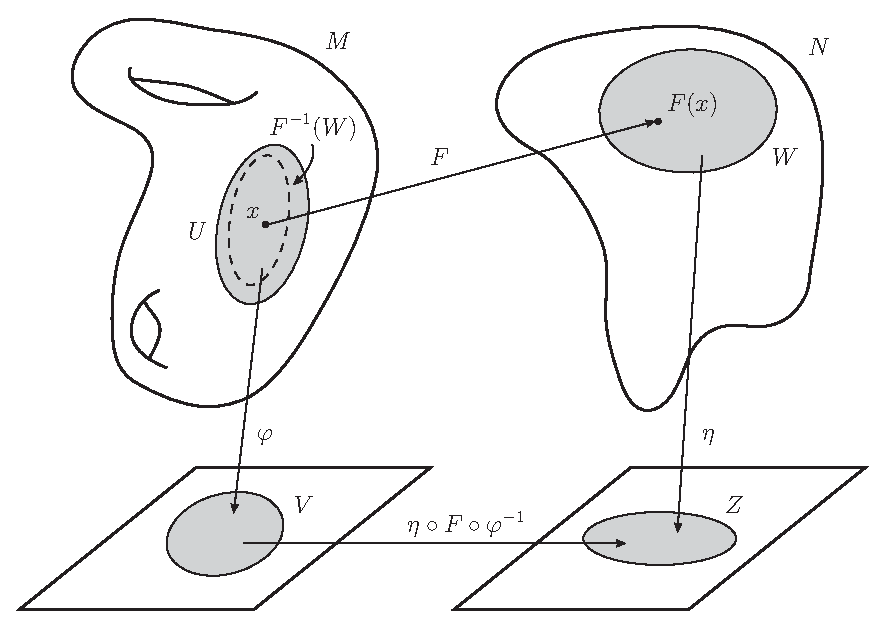
\includegraphics[scale=0.7]{fig/mani-map-1b}
\caption{A map between manifolds.}
\label{fig:mani-map-1}
\end{figure}

\subsubsection{Submanifolds}
%\texttt{Maybe use different definition?}
\begin{definition}
A subset $M$ of $\mathbb{R}^n$ is a $k$-dimensional \textit{submanifold} if for all points $x\in M$, there exists a neighbourhood $V$ of $x\in\mathbb{R}^n$, an open set $U\subseteq\mathbb{R}^k$ and a smooth map $\xi:U\to\mathbb{R}^n$ such that $\xi$ is a homeomorphism onto $M\cap V$ and $D_y\xi$ is injective for all $y\in U$. 
\end{definition}
Even though we have not yet explicitly defined what we mean by the differential of a map, $D_y\xi$, the last statement in the above definition can be interpreted as requiring continuity with respect to the `subspace topology' on $M$ induced from the inclusion into $\mathbb{R}^n$. Since open sets in the subspace topology are given by restrictions of open sets in $\mathbb{R}^n$, this is equivalent to the statement that given any open set $A\subseteq U$, there is an open set $B\subseteq\mathbb{R}^n$, such that $\xi(A)=M\cap B$.
\subsection{Tangent Spaces}
%Talk for a bit...

In this section we will give three different ways of thinking about the tangent space to a point of an abstract manifold and then show that these three characterisations are in fact equivalent.

Let $M$ be a smooth $n$-dimensional manifold. The first characterisation goes as follows. For any $x\in M$, define $T_xM$ to be the set of pairs $(\varphi,u)$ where $\varphi:U\to V$ is a chart in the atlas for $M$ with $x\in U$ and $u\in\mathbb{R}^n$, modulo the equivalence relation which identifies a pair $(\varphi,u)$ with a pair $(\eta,w)$ if and only if $u$ maps to $w$ under the derivative of the transition map between the two charts $\varphi$ and $\eta$,
\[
D_{\varphi(x)}(\eta\circ\varphi^{-1})(u)=w.
\]
The second characterisation comes about by considering what the idea of a `velocity vector' in a manifold could mean. Define $M_x$ to be space of smooth paths in $M$ through $x$. By smooth path through $x$ we mean a smooth map $\gamma:[a,b]\to M$, such that $\gamma(0)=x$. Now consider $M_x$ modulo the equivalence relation which identifies any two curves if they have the same derivative, i.e. 
\[
\gamma\sim\sigma\Leftrightarrow(\varphi\circ\gamma)'(0)=(\varphi\circ\sigma)'(0),
\] 
for some chart $\varphi:U\to V$ with $x\in U$. 

This idea is schematically illustrated below in Figure \ref{fig:tang-1}. 

\begin{figure}[h!]
\centering
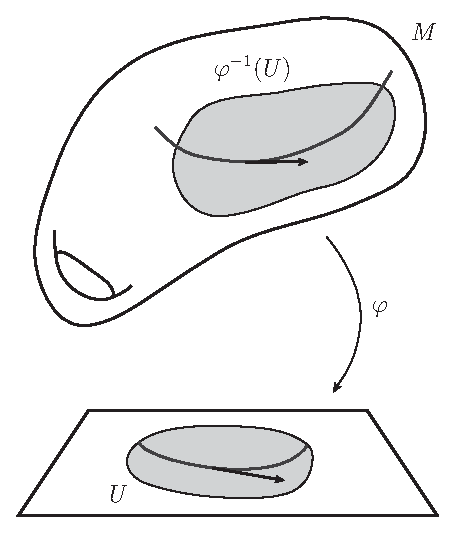
\includegraphics[scale=0.75]{fig/tang-3b}
\caption{A tangent vector to $x$ defined by a curve through $x$.}
\label{fig:tang-1}
\end{figure}

Before describing the third characterisation of tangent vectors, we have the following definition.
\begin{definition}
\label{def:derivation}
A \textit{derivation} at $x$ is a map $v:C^{\infty}(M)\to\mathbb{R}$ such that for any smooth functions $f,g$ on $M$ and real numbers $c_1,c_2$,
\begin{align*}
v(c_1f+c_2g)&=c_1v(f)+c_2v(g)\\
v(fg)&=f(x)v(g)+g(x)v(f).
\end{align*}
The first condition is simply that $v$ is linear and the second condition is known as the Leibniz identity.
\end{definition}
One of the most common examples of a derivation is the directional derivative of a function along a curve. Given a smooth path $\gamma:[a,b]\to M$ with $\gamma(0)=x$, we can compute,
\begin{equation}
v(f)=\left.\frac{d}{dt}(f\circ\gamma)\,\right\rvert_{t=0},
\label{eq:derivation-dirderiv}
\end{equation}
which defines a derivation at $x$. We can then define $D_xM$ as the space of all derivations through $x$, which is the third characterisation of the tangent space at $x$.

As stated at the beginning of the section, we can show that these three definitions of the tangent space of a point in $M$ are in fact equivalent.
\begin{proposition}
There are natural isomorphisms between the three spaces $M_x$, $T_xM$ and $D_xM$.
\[
\begin{tikzcd}[column sep=small]
T_xM \arrow{rr}{\alpha} && M_x\arrow{dl}{\beta}\\
&D_xM\arrow{ul}{\chi}
\end{tikzcd}
\]
\end{proposition}
\begin{proof}
First, given an equivalence class $[(\varphi,u)]$ in $T_xM$, take $\alpha([(\varphi,u)])$ to be the equivalence class of the smooth path given by
\[
\gamma(t)=\varphi^{-1}(\varphi(x)+tu).
\]
We have that $\alpha$ is well-defined, since if $(\eta,w)$ is another representative of the same equivalence class in $T_xM$, then $\alpha$ gives the equivalence class of the curve $\sigma(t)=\eta^{-1}(\eta(x)+tw)$ and we get,
\begin{align*}
(\varphi\circ\sigma)'(0)&=\left((\varphi\circ\eta^{-1})\circ(\eta\circ\sigma) \right)'(0)\\
&=D_{\eta(x)}\left(\varphi\circ\eta^{-1} \right)(\eta\circ\sigma)'(0)\\
&=D_{\eta(x)}\left(\varphi\circ\eta^{-1}\right)(w)\\
&=u\\
&=(\varphi\circ\gamma)'(0),
\end{align*}
and so $[\sigma]=[\gamma]$.

Now, given some $[\gamma]\in M_x$, take $\beta([\gamma])$ to be the natural derivation $v$ given by \eqref{eq:derivation-dirderiv}. We check this is well-defined as follows. Suppose $[\sigma]=[\gamma]$ and $f$ is some smooth function. Then we have,
\begin{align*}
\left.\frac{d}{dt}(f\circ\gamma)\,\right\rvert_{t=0}&=\left.\frac{d}{dt}\left[(f\circ\varphi^{-1})\circ(\varphi\circ\gamma) \right]\right\rvert_{t=0}\\
&=D_{\varphi(x)}(f\circ\varphi^{-1})(\varphi\circ\gamma)'(0)\\
&=D_{\varphi(x)}(f\circ\varphi^{-1})(\varphi\circ\sigma)'(0)\\
&=\left.\frac{d}{dt}(f\circ\sigma)\,\right\rvert_{t=0},
\end{align*}
as required.

Next, given some derivation $v$, choose a chart $\varphi$ containing $x$ and take $\chi(v)$ to be the element of $T_xM$ given by taking the equivalence class $[(\varphi,u)]$ such that $u=\left(v(\varphi^1),\ldots,v(\varphi^n)\right)$, where $\varphi^i$ is the $i$th component function of the chart $\varphi$.\\

Note the following technicality. Definition \ref{def:derivation} says that derivations must act on smooth functions defined on all of $M$, but the $\varphi^i$ are only defined on an open set $U$ of $M$. This issue is addressed by extending the $\varphi^i$ to give a smooth map defined on all of $M$. Let us define the following functions.
\begin{equation}
\xi(z)=\begin{cases}
\exp(\frac{1}{z^2-1}) & |z|<1\\
0 & |z|\geq 1
\end{cases},
\label{eq:bumpf-1}
\end{equation}
and
\begin{equation}
\rho(z)=\frac{\int_{-1}^z\xi(t)\,dt}{\int_{-1}^{1}\xi(t)\,dt}.
\label{eq:rampf-1}
\end{equation}
We have that $\xi$ is a smooth function of all of $\mathbb{R}$, with $\xi(z)>0$ on the interval $(-1,1)$ and zero otherwise. In addition, $\rho$ is a smooth function on all of $\mathbb{R}$ which is zero for $z\leq -1$, strictly increasing on the interval $(-1,1)$ and precisely one for $z>1$.

\begin{figure}[h!]
\centering
\begin{subfigure}[b]{0.5\textwidth}
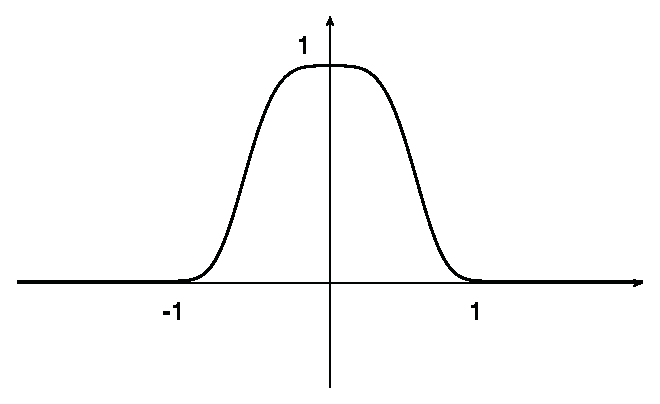
\includegraphics[scale=0.55]{fig/bump-1c}
\caption{A smooth `bump' function $\xi$.}
\end{subfigure}%
\begin{subfigure}[b]{0.5\textwidth}
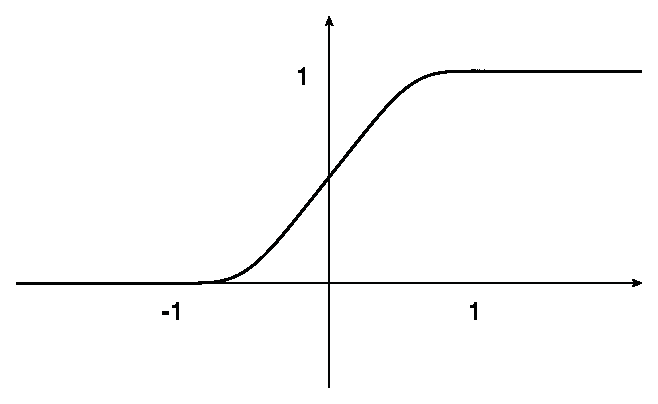
\includegraphics[scale=0.55]{fig/ramp-1c}
\caption{A smooth `ramp' function $\rho$.}
\end{subfigure}
\caption{Graphs of the functions defined by $\xi$ and $\rho$ respectively.}
\label{fig:bump-n-ramp}
\end{figure}

Given a chart $\varphi:U\to V$ with $x\in U$, choose some $\varepsilon$ sufficiently small enough to ensure that the closed ball of radius $4\varepsilon$ about $\varphi(x)$ is contained in $V$. Then define $\tilde{\rho}$ on $M$ by
\begin{equation}
\tilde{\rho}(y)=\begin{cases}
\rho\left( 3-\frac{|\varphi(y)-\varphi(x)|}{\varepsilon} \right) & y\in U,\\
0 & y\in M\backslash U.
\end{cases}
\label{eq:tilde-rho}
\end{equation}
This construction gives a function $\tilde{\rho}$ which is identically equal to one on a neighbourhood of $x$ and identically zero in the complement of a larger neighbourhood.\\

If $f:U\to\mathbb{R}$ is a smooth function on an open set $U$ of $M$ containing $x$, define $v(f)=v(\tilde{f})$ where $\tilde{f}$ is any smooth function on $M$ which agrees with $f$ on a neighbourhood of $x$.\\

We check that such a smooth function $\tilde{f}$ on $M$ which agrees with $f$ on a neighbourhood of $x$ does not depend on which function we choose as follows.

Without loss of generality, suppose $f$ is defined on $U$ as before and define $\tilde{\rho}$ as per \eqref{eq:tilde-rho}. Then define,
\begin{equation}
\tilde{f}(y)=\begin{cases}
f(y)\tilde{\rho}(y) & y\in U\\
0 & y\in M\backslash U
\end{cases},
\end{equation}
which is smooth and agrees with $f$ on the set $\varphi^{-1}\left( B_{2\varepsilon}(\varphi(x)) \right)$.\\

We verify that $v(\tilde{f})$ does not change if we choose a different function agreeing with $f$ on a neighbourhood of $x$.
\begin{lemma}
Let $f,g$ be two smooth functions on $M$ which agree on a neighbourhood of $x$. Then $v(f)=v(g)$.
\end{lemma}
\begin{proof}
Without loss of generality, suppose that $f$ and $g$ agree on an open set $U$ containing $x$ and construct a bump function $\tilde{\rho}$ in $U$ as before. Observe that $\tilde{\rho}(f-g)$ is identically zero on $M$ and that $v(0)=v(0\cdot 0)=0\cdot v(0)=0$. Hence, we have,
\[
0=v(\tilde{\rho}(f-g))=\tilde{\rho}(x)v(f-g)+(f(x)-g(x))v(\tilde{\rho})=v(f)-v(g),
\]
since $f(x)-g(x)=0$ and $\tilde{\rho}(x)=1$.
\end{proof}
Thus, the posited definition of $v(f)$ has been shown to be consistent with the definition of $\chi(v)$, and is hence is well defined. However, it remains to be checked that $\chi(v)$ is independent of our choice of a chart $\varphi$. Suppose we have another chart $\eta$. Then in a small region about $x$,
\begin{equation}
\eta^i(y)=\eta^i(x)+\sum_{j=1}^nG^i_j(y)\left( \varphi^j(y)-\varphi^j(x) \right),
\end{equation} 
for $i=1,\ldots,n$ and where $G^i_j$ is a smooth function on a neighbourhood of $x$ such that
\[
G^i_j(x)=\frac{\partial}{\partial x^j}\left.\left(\eta^i\circ\varphi^{-1}\right)\,\right\rvert_{\varphi(x)}.
\]
%\texttt{Details needed?}

Applying $v$ to $\eta^i$ yields,
\begin{align*}
v(\eta^i)&=\sum_{j=1}^n G^i_j(x)v(\varphi^j)+(\varphi^j(x)-\varphi^i(x))v(G^i_j)\\
&=\sum_{j=1}^{n}\frac{\partial}{\partial x^j}\left.\left(\eta^i\circ\varphi^{-1}\right)\,\right\rvert_{\varphi(x)}v(\varphi^j).
\end{align*}
We hence have,
\begin{align*}
\sum_{i=1}^n v(\eta^i)e_i&=\sum_{i,j=1}^n\frac{\partial}{\partial x^j}\left.\left(\eta^i\circ\varphi^{-1}\right)\,\right\rvert_{\varphi(x)}v(\varphi^j)e_i\\
&=D_{\varphi(x)}(\eta\circ\varphi^{-1})\left( \sum_{i=1}^nv(\varphi^i)e_i \right),
\end{align*}
and so $\left[ (\varphi,\sum_{i=1}^nv(\varphi^i)e_i )\right]=\left[(\eta,\sum_{i=1}^nv(\eta^i)e_i) \right]$. Thus $\chi$ is independent of the choice of chart.

It now suffices to show that $\chi\circ\beta\circ\alpha$, $\alpha\circ\chi\circ\beta$ and $\beta\circ\alpha\circ\chi$ all give the identity map on each of the three spaces.

We have the following.
\begin{align*}
\chi\circ\beta\circ\alpha([(\varphi,u)])&=\chi\circ\beta\left(\left[t\mapsto\varphi^{-1}(\varphi(x)+tu) \right] \right)\\
&=\chi\left(f\mapsto D_{\varphi(x)}(f\circ\varphi^{-1})(u) \right)\\
&=\left[ \left( \varphi,\sum_{i=1}^{n}D_{\varphi(x)}(\varphi^i\circ\varphi^{-1})(u)e_i \right) \right]\\
&=[(\varphi,u)].
\end{align*}
Next we have,
\begin{align*}
\alpha\circ\chi\circ\beta([\sigma])&=\alpha\circ\chi\left(f\mapsto\left.\frac{d}{dt}(f\circ\gamma)\,\right\rvert_{t=0} \right)\\
&=\alpha\left( \left[ \left( \varphi,\sum_{i=1}^{n}(\varphi\circ\gamma)'(0) \right) \right] \right)\\
&=\left[t\mapsto\varphi^{-1}(\varphi(x)+t(\varphi\circ\gamma)'(0)) \right],
\end{align*}
which is a curve in the same equivalence class as $\gamma$.

Finally,
\begin{align*}
\beta\circ\alpha\circ\chi(v)&=\beta\circ\alpha\left( \left[ \left( \varphi,\sum_{i=1}^{n}v(\varphi^i)e_i \right) \right] \right)\\
&=\beta\left( \left[ t\mapsto \varphi^{-1}\left( \varphi(x)+t\sum_{i=1}^nv(\varphi^i)e_i \right) \right] \right)\\
&=\left( f\mapsto\sum_{i=1}^n\frac{\partial}{\partial x^i}\left.(f\circ\varphi^{-1})\,\right\rvert_{\varphi(x)}v(\varphi^i) \right).
\end{align*}
To show that this is the same as $v$ as we require, consider the following result. Via a Taylor expansion for $f\circ\varphi^{-1}$, we have that
\[
f(y)=f(x)+\sum_{i=1}^nG_i(y)\left(\varphi^i(y)-\varphi^i(x)\right),
\]
for $y$ in a sufficiently small neighbourhood of $x$ and where $G_i$ is a smooth function such that $G_i(x)=\frac{\partial}{\partial x^i}\left. (f\circ\varphi^{-1})\,\right\rvert_{\varphi(x)}$. Applying $v$ to this expression yields,
\begin{equation}
v(f)=\sum_{i=1}^{n}G_i(x)v(\varphi^i)=\sum_{i=1}^n\frac{\partial}{\partial x^i}\left.(f\circ\varphi^{-1})\,\right\rvert_{\varphi(x)}v(\varphi^i),
\label{eq:vf-detail-1}
\end{equation}
the right hand side of which is the same as $\beta\circ\alpha\circ\chi(v)$, as required.
%\begin{center}
%\texttt{Details to be filled in...}
%\end{center}
\end{proof}
Having now established the equivalence of $M_x$, $T_x$ and $D_xM$, we shall now simply use the notation $T_xM$ to refer to the tangent space to $x$ at $M$ while using any of the three different characterisations of a tangent vector depending on what best suits the task at hand.
\subsubsection{The Differential of a Map}
\begin{definition}
Let $f:M\to\mathbb{R}$ be a smooth function. We define the differential $d_xf$ of $f$ at the point $x\in M$ to be the linear function on $T_xM$ given by $(d_xf)(v)=v(f)$ for all $v\in T_xM$, where we are considering $v$ as a derivation. 

%Let $F:M\to N$ be a smooth map between manifolds. Define the differential $D_xF$ of $F$ at $x\in M$ to be the linear map from $T_xM$ to $T_{F(x)}N$ given by $\left((d_xF)(v) \right)(f)=v(f\circ F)$ for any $v\in T_xM$ and $f\in C^{\infty}(M)$.
Let $F:M\to N$ be a smooth map between manifolds $M$ and $N$. For all points $x\in M$, define the map
\[
D_xF:T_xM\to T_{F(x)}N,
\]
to be the \textit{differential of $F$ at $x$} as follows. Given a tangent vector $v\in T_xM$, let $D_xF(v)$ be the derivation at $F(x)$ that acts on $f\in C^{\infty}(N)$ by the rule
\[
D_xF(v)(f)=v(f\circ F).
\]
\end{definition}
Alternatively, if one thinks of a vector $v$ as the tangent vector to a curve $\gamma$, then we have
\[
D_xF(v)=(F\circ\gamma)'(0),
\] 
for any smooth curve $\gamma$ such that $\gamma(0)=x$ and $\gamma'(0)=v$.
%\texttt{More detail needed?}

\begin{figure}[h!]
\centering
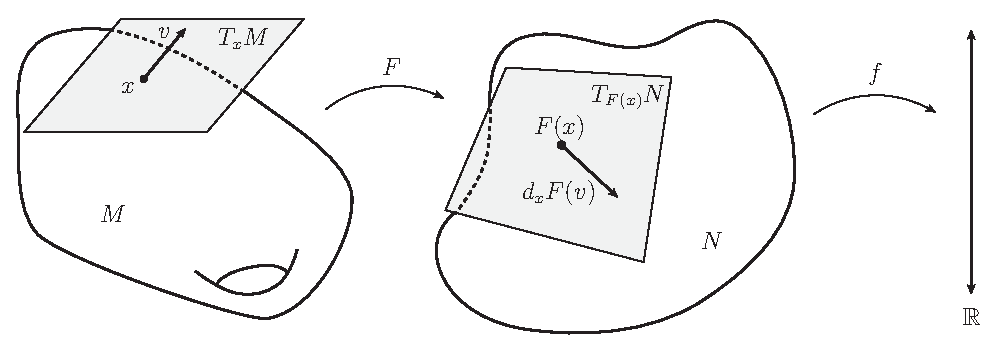
\includegraphics[scale=0.75]{fig/differential-1b}
\caption{The differential of a map $F:M\to N$.}
\label{fig:diff-1}
\end{figure}
\begin{definition}
If $F:M\to N$ is a smooth map, a point $x\in M$ is said to be a \textit{regular point of $F$} if $D_xF:T_xM\to T_{F(x)}N$ is surjective. A point $y\in N$ is said to be a \textit{regular value of $F$} is every point of the preimage $F^{-1}(y)$ is a regular point.
\end{definition}
%$v:f\mapsto (f\circ\gamma)'(0)$ and so the differential of a map $F:M\to N$ is given by the assignment,
%\[
%d_xF(v):f\mapsto (f\circ F\circ\gamma)'(0),
%\] 
%which is the tangent vector of the curve $F\circ \gamma$. This is then to say,
%\[
%d_xF([\gamma])=[F\circ\gamma].
%\]
\subsubsection{Coordinate Tangent Vectors}
We now consider how computations with tangent vectors and differentials can be carried out in local coordinates.

Let $\varphi:U\to V$ be a chart on a smooth manifold $M$ with $x\in U$. One can construct a basis for $T_xM$ by simply taking the vectors corresponding to the equivalence classes $[(\varphi,e_i)]$, where $e_1,\ldots,e_n$ are the standard basis vectors in $\mathbb{R}^n$. 

We shall adopt the notation $\partial_i=[(\varphi,e_i)]$, without explicitly referring to a chart $\varphi$. Considering this as a derivation, we have that $\partial_if=\left.\frac{\partial}{\partial x^i}(f\circ\varphi^{-1})\right\rvert_{\varphi(x)}$. This is to say, $\partial_i$ is simply the derivation given by taking the $i$th partial derivative in the coordinates defined by $\varphi$. By Proposition 2.2, it follows that $\{\partial_1,\ldots,\partial_n\}$ is a basis for $T_xM$.
%\texttt{The differential in coordinates?}
\subsection{Vector Bundles}
%\texttt{Where to put this section...}
\begin{definition}
A real \textit{vector bundle} of rank $k$ is a triple $(M,E,\pi)$. Where $M$ is a smooth manifold called the base space, $E$ is a smooth manifold called the total space and $\pi:E\to M$ is a smooth surjection called the projection. We also impose the following conditions on $\pi$.
\begin{enumerate}[(i)]
\item For all points $x\in M$, the fibre $E_x=\pi^{-1}(x)$ over $x$ is endowed with the structure of a $k$-dimensional vector space.
\item For all $x\in M$, there exists a neighbourhood $U$ of $x$ in $M$ and a homeomorphism $\psi:\pi^{-1}(U)\to U\times\mathbb{R}^k$, called the \textit{local trivialisation of $E$ over $U$}, such that:
\begin{itemize}
\item $\pi_U\circ\psi=\pi$ where $\pi_U:U\times\mathbb{R}^k\to U$ is the projection;
\item for all $q\in U$, the restriction of $\psi$ to $E_q$ is a vector space isomorphism from $E_q$ to $\{q\}\times\mathbb{R}^k\cong\mathbb{R}^k$.
\item on the intersection $U\cap V$ we have
\[
\psi_U\psi^{-1}_V:U\cap V\times\mathbb{R}^k\to U\cap V\times\mathbb{R}^k,
\]
is of the form,
\[
(x,v)\mapsto\left(x,g_{UV}(x)v\right),
\]
where $g_{UV}:U\cap V\to\mathrm{GL}(k)$.
\end{itemize}
\end{enumerate}
In an abuse of notation, we will often simply refer to a vector bundle by the map $\pi:E\to M$ since it references all elements of the formal triple $(E,M,\pi)$. 
\end{definition}

Figure \ref{fig:bundle-1} illustrates the basic concept of a vector bundle, highlighting a local trivialisation.

\begin{figure}[h!]
\centering
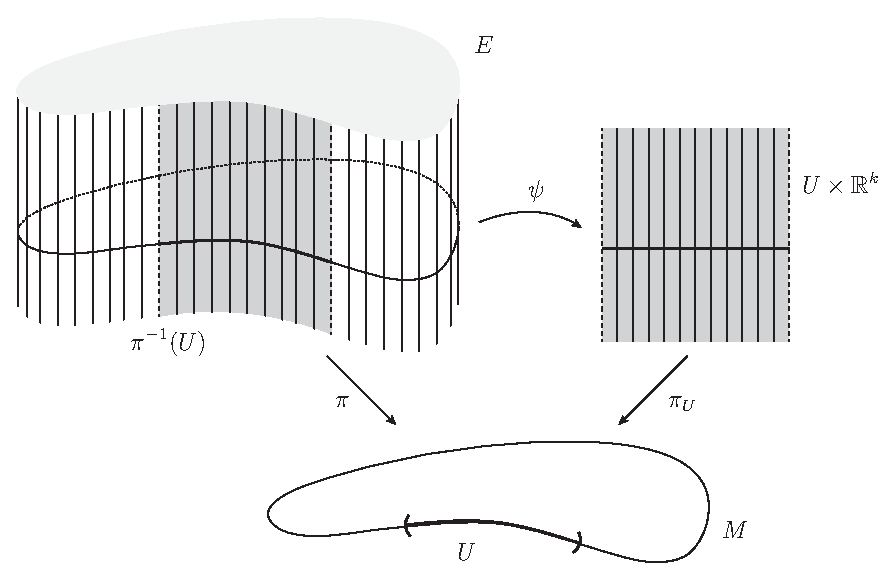
\includegraphics[scale=0.75]{fig/bundle-2b}
\caption{Sketch of a vector bundle.}
\label{fig:bundle-1}
\end{figure}

\begin{definition}
A \textit{section} of a vector bundle $\pi:E\to M$ is a continuous map $\sigma:M\to E$ satisfying $\pi\circ\sigma=\mathrm{id}_M$. This is to say that, $\sigma(x)$ is an element of the fibre $E_x$, for all points $x\in M$. A \textit{local section} is a section $\sigma$ defined on some open subset $U\subset M$. If $U=M$ then $\sigma$ is sometimes referred to as a \textit{global section}.
\end{definition}

\begin{figure}[h!]
\centering
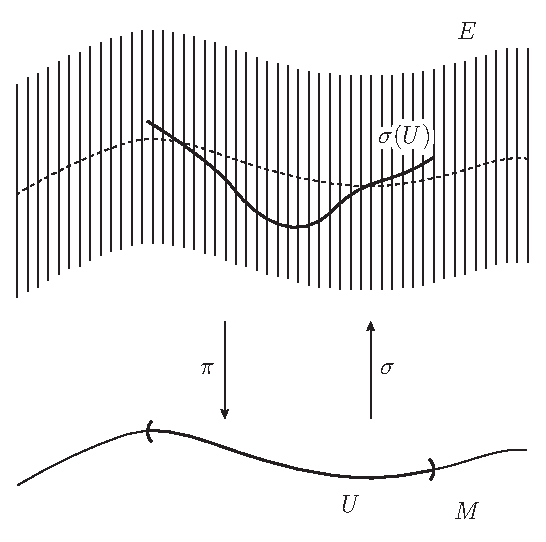
\includegraphics[scale=0.75]{fig/section-1}
\caption{Diagram illustrating a section of a vector bundle.}
\label{fig:section-1}
\end{figure}

\subsubsection{The Tangent Bundle}
It is often useful to consider the set of all tangent spaces to all points of a manifold. As such, we now consider a concrete example of a vector bundle which is of fundamental importance for this project, this being the tangent bundle of a manifold.

\pagebreak

\begin{definition}
The \textit{tangent bundle} of a manifold $M$, denoted by $TM$, is the disjoint union of the tangent spaces at all points of $M$,
\[
TM=\bigsqcup_{x\in M}T_xM=\{(x,v):x\in M,v\in T_xM\}.
\]
In terms of our definition of a vector bundle, we have $M$ as the base space, $TM$ as the total space and $\pi:TM\to M$, given by $\pi(x,v)=x$, which sends each vector in $T_xM$ to the point $x$ at which it is tangent. Furthermore, observe that
\[
(x,v)\mapsto \left(\psi\circ\varphi^{-1}(x),d(\psi\circ\varphi^{-1})v \right),
\]
gives us a vector bundle structure since $d(\psi\circ\varphi^{-1})$ is linear.
\end{definition}
If $M$ has dimension $n$, then we can endow the tangent bundle $TM$ with the structure of a $2n$-dimensional manifold. Given a chart $\varphi:U\to V$ for $M$, define a chart $\tilde{\varphi}$ for $TM$ on the set $\pi^{-1}(U)=\{(x,v)\in TM:x\in U\}$ by,
\[
\tilde{\varphi}(x,v)=\left(\varphi(x),v(\varphi^1),\ldots,v(\varphi^n) \right)\in\mathbb{R}^{2n}.
\]
The first $n$ coordinates describe the point $x$ and the last $n$ given the components of the vector $v$ with respect to the basis of the coordinate tangent vector $\{\partial_i\}_{i=1}^{n}$. From Equation \eqref{eq:vf-detail-1}, we have the following description of the local coordinate expression for $v$,
\[
v(f)=\sum_{i=1}^n\frac{\partial}{\partial x^i}\left.\left(f\circ\varphi^{-1}\right)\,\right\rvert_{\varphi(x)}v(\varphi^i)=\sum_{i=1}^nv(\varphi^i)\partial_i(f),
\]
with $f\in C^{\infty}(M)$. Hence we can write $v=\sum_{i=1}^nv(\varphi^i)\partial_i$.

To show that these charts give $TM$ a manifold structure, it suffices to compute the transition maps. Refer to \cite{MR2954043} for the explicit computation of this.

%Suppose we are given two charts $\varphi:U\to V$ and $\eta:W\to Z$ such that their intersection is non-empty.
%\begin{center}
%\texttt{Details to be filled in...}
%\end{center}

\begin{definition}[Bundle Morphism]
If $\pi:E\to M$ and $\pi':E'\to M'$ are vector bundles, a continuous map $F:E\to E'$ is a \textit{bundle morphism} (or \textit{bundle homomorphism}), if there exists a map $f:M\to M'$ such that $f\circ\pi=\pi'\circ F$,
\[
\begin{tikzcd}
E \arrow[r,"F"] \arrow{d}[swap]{\pi}
& E' \arrow[d,"\pi'"] \\
M \arrow{r}[swap]{f} & M'
\end{tikzcd}
\]
with the property that for all $x\in M$, the restricted map $F\rvert_{E_x}:E_x\to E'_{f(x)}$ is linear.

A bijective bundle homomorphism $F:E\to E'$ whose inverse is also a bundle homomorphism is called a \textit{bundle isomorphism}.
\end{definition}

\begin{example}
If $F:M\to N$ is a smooth map between manifolds $M$ and $N$ then the global differential $dF:TM\to TN$ is a smooth bundle homomorphism.
\end{example}

Let $\pi:E\to M$ be a vector bundle. If $U\subseteq M$ is an open subset, a $k$-tuple of local section $(\sigma_1,\ldots,\sigma_k)$ of $E$ over $U$ is linearly independent if $(\sigma_1(x),\ldots,\sigma_k(x))$ is linearly independent $k$-tuple in $E_x$ for all $x\in U$. Similarly, they are said to span $E$ if their values span $E_x$ for all $x\in U$.

\begin{definition}
A \textit{local frame} for $E$ over $U$ is an ordered $k$-tuple $(\sigma_1,\ldots,\sigma_k)$ of linearly independent local sections over $U$ that span $E$, i.e. $(\sigma_1(x),\ldots,\sigma_k(x))$ is a basis for the fibre $E_x$ for each $x\in U$.

If $U=M$ then it is said to be a \textit{global frame}.
\end{definition}
\begin{example}
Let $E:M\times\mathbb{R}^n\to M$ be a vector bundle. The standard basis $(e_1,\ldots,e_n)$ for $\mathbb{R}^n$ yields a global frame $(\tilde{e}_i)$ for $E$ given by $(\tilde{e}_i)(x)=(x,e_i)$.
\end{example}
\begin{example}
Let $\pi:E\to M$ be a vector bundle. If $\phi:\pi^{-1}(U)\to U\times \mathbb{R}^n$ is a local trivialisation of $E$, we can use the same technique as in the previous example to construct a local frame for $E$ over $U$. Define maps $\sigma_1,\ldots,\sigma_n: U\to E$ by $\sigma_i(x)=\phi^{-1}(x,e_i)=\phi^{-1}\circ\tilde{e}_i(x)$,
\[
\begin{tikzcd}[column sep=small]
\pi^{-1}(U) \arrow{dr}{\pi} \arrow{rr}{\phi} && U\times\mathbb{R}^n \arrow{dl}[swap]{\pi_1}\\
&U \arrow[ul, bend left, "\sigma_i"] \arrow[ur, bend right,swap,"\tilde{e}_i"]
\end{tikzcd}.
\]

The fact that $\pi_1\circ\phi=\pi$ implies that,
\[
\pi\circ\sigma_i(x)=\pi\circ\phi^{-1}(x,e_i)=\pi_1(x,e_i)=x,
\]
and so $\sigma_i$ is a section.

To see that $(\sigma_i(x))$ forms a basis for $E_x$, observe that $\phi$ restricts to an isomorphism from $E_x$ to $\{x\}\times\mathbb{R}^n$ and $\phi(\sigma_i(x))=(x,e_i)$, so $\phi$ takes $(\sigma_i(x))$ to the standard basis for $\{x\}\times\mathbb{R}^n\cong\mathbb{R}^n$.
\end{example}
In the above example, we say that the local frame $(\sigma_i)$ is \textit{associated with $\phi$}.
\begin{proposition}
Every local frame for a vector bundle is associated with a local trivialisation.
\label{vb-lf-lt}
\end{proposition}
\begin{proof}
Suppose $\pi:E\to M$ is a vector bundle and $(\sigma_i)$ is a local frame for $E$ over some open subset $U\subseteq M$. Define a map $\psi:U\times\mathbb{R}^n\to\pi^{-1}(U)$ by
\[
\psi(x,(v^1,\ldots,v^n))=v^i\sigma_i(x).
\]
From the fact that $(\sigma_i(x))$ forms a basis for $E_x$ at each point $x\in U$, we get that $\psi$ is bijective and furthermore that $\sigma_i=\psi\circ\tilde{e}_i$. Hence, if we show that $\psi$ is a diffeomorphism, then $\psi^{-1}$ will be a local trivialisation whose associated local frame is $(\sigma_i)$.

Since $\psi$ is bijective, it suffices to show that it is a local diffeomorphism. Given $y\in U$, we can find a neighbourhood $V$ of $x$ in $M$ over which there exists a local trivialisation $\phi:\pi^{-1}(V)\to V\times\mathbb{R}^n$ and by scaling $V$ if necessary, we may assume that $V\subseteq U$. Since $\phi$ is a diffeomorphism, if we show that $\phi\circ\psi\rvert_{V\times\mathbb{R}^n}$ is a diffeomorphism from $V\times\mathbb{R}^n$ to itself, it follows that $\psi$ restricts to a diffeomorphism from $V\times\mathbb{R}^n$ to $\pi^{-1}(V)$, as shown in the following diagram.
\[
\begin{tikzcd}
V\times\mathbb{R}^n\arrow{dr}[swap]{\pi_1} \arrow{r}{\psi\rvert_{V\times\mathbb{R}^n}} & \pi^{-1}(V) \arrow{r}{\phi} \arrow{d}{\pi} & V\times\mathbb{R}^n \arrow{dl}{\pi_1}\\
& V
\end{tikzcd}
\]
For each of the smooth sections $\sigma_i$, the composite map $\phi\circ\sigma_i\rvert_V:V\to V\times\mathbb{R}^n$ is smooth and hence there are smooth functions $\sigma^1_i,\ldots,\sigma^n_i:V\to\mathbb{R}$ such that
\[
\phi\circ\sigma_i(x)=\left(x,\left(\sigma^1_i(x),\ldots,\sigma^n_i(x) \right) \right).
\]
Thus, on $V\times\mathbb{R}^n$ we have,
\[
\varphi\circ\psi\left(x,(v^1,\ldots,v^n) \right)=\left(x,\left(v^i\sigma^1_i(x),\ldots,v^i\sigma^n_i(x) \right) \right),
\]
which is a composition of smooth functions and so is itself smooth.

To show $(\phi\circ\psi)^{-1}$ is smooth, note that the matrix $(\sigma^j_i(x))$ is invertible for all $x$ since $(\sigma_i(x))$ is a basis for $E_x$. Let $(\tau^j_i(x))$ denote the inverse matrix. Since matrix inversion is a smooth map from $\mathrm{GL}(n,\mathbb{R})$ to itself, the functions $\tau^j_i$ are smooth. It follows from the above computations that
\[
(\phi\circ\psi)^{-1}\left(x,(w^1,\ldots,w^n)\right)=\left(x,\left(w^i\tau^1_i(x),\ldots,w^i\tau^n_i(x) \right) \right),
\]
is a smooth function which completes the proof.
\end{proof}
\begin{corollary}
A vector bundle is trivial if and only if it admits a global frame.
\end{corollary}
\begin{proof}
From the previous examples and Proposition \ref{vb-lf-lt}, we have that there is a local trivialisation over an open subset $U\subseteq M$ if and only if there is a local frame over $U$. The corollary is simply the special case of Proposition \ref{vb-lf-lt} when $U=M$.
\end{proof}
\pagebreak
\subsection{Vector Fields}
\begin{definition}
If $M$ is a smooth manifold, a \textit{vector field on $M$} is a section of the tangent bundle, $X:M\to TM$. By definition of a section, if $\pi:TM\to M$ is the natural projection map of the tangent bundle, then
\[
\pi\circ X=\mathrm{id}_M.
\] 
In local coordinates we have,
\[
X(x_1,\ldots,x_n)=(x_1,\ldots,x_n,X^1(x),\ldots,X^n(x)),
\]
where the $X^i(x)$ are smooth functions. Hence the tangent vector $X(x)$ is given by,
\begin{equation}
X_x=\sum_iX^i(x)\left(\frac{\partial}{\partial x^i}\right)_x,
\label{eq:vect-local}
\end{equation}
which is a smoothly varying field of tangent vectors.
\end{definition}
From our definition of tangent vectors in terms of derivations, we also have the following proposition which allows us to describe vector fields in terms of derivations.
\begin{proposition}
Let $X:C^{\infty}(M)\to C^{\infty}(M)$ be a linear map which satisfies the Leibniz identity,
\[
X(fg)=f(Xg)+g(Xf).
\]
Then $X$ is a vector field.
\end{proposition}
\begin{proof}
Given such a derivation $X$ and $x\in M$, the map $X_x:C^{\infty}(M)\to\mathbb{R}$ given by $X_x(f)=(X(f))(x)$ is a derivation at $x$ and so defines an element of $T_xM$. The map $x\mapsto X_x$ from $M$ to $TM$ is hence a vector field and it remains to check smoothness. The components of $X_x$ with respect to the coordinate tangent basis $\partial_1,\ldots,\partial_n$ for a chart $\varphi:U\to V$ is given by,
\[
X_x^i=X_x(\varphi^i),
\]
which is by assumption a smooth function of $x$ for each $i$ (since $\varphi^i$ is a smooth function and $V$ maps smooth functions to smooth functions). We can extend the $\varphi^i$ by a bump function such as the one given by Equation \eqref{eq:bumpf-1} in a coordinate neighbourhood to convert it to a smooth function on the whole of $M$. Hence the vector field is smooth.

Conversely, given a smooth vector field $x\mapsto X_x\in T_xM$, the map,
\[
(X(f))(x)=X_x(f),
\] 
satisfies the conditions necessary for a derivation and takes a smooth function to a smooth function.
%For all $x\in M$, $X_x(f)$ satisfies the conditions for a tangent vector at $x$, and so $X$ defines a map $X:M\to TM$ with $\pi\circ X=\mathrm{id}_M$ and can be written locally in the form of Equation \eqref{eq:vect-local}.
%
%It suffices to show that the $y_i(x)$ are smooth, and for this we simply need to apply $X$ to a coordinate function $x_i$ extended by a bump function \texttt{should probably define this earlier on somewhere eh?} in a coordinate neighbourhood. This is simply,
%\[
%Xx_i=y_i(x),
%\]
%and since by assumption $X$ maps smooth functions to smooth functions, the $y_i(x)$ are smooth.
\end{proof}
\begin{remark}
In this report, we are interested in \textit{nowhere vanishing} vector fields on spheres. By this, it is meant that given some vector field $X$ on $\mathbb{S}^n$, we want $X(x)\neq 0$ for any given point $x\in\mathbb{S}^n$.
\end{remark}
\subsection{Differential Forms}
%\textbf{\textcolor{red}{Might have to go unused...}}\\
In order to build up to the notion of a differential form, we have the following definitions.
\begin{definition}
A \textit{covector} $\omega$ at $x\in M$ is a linear map from $T_xM$ to $\mathbb{R}$. The set of covectors at $x$ form an $n$-dimensional vector space denoted by $T^*_xM$ (in the language of linear algebra, this is the dual space to $T_xM$).
\end{definition}
\begin{definition}
A \textit{tensor} of type $(k,l)$ at $x$ is a multilinear map $T_x$ which takes $k$ vectors and $l$ covectors and returns a real number,
\[
T_x:\underbrace{T_xM\times\cdots\times T_xM}_{k\text{ copies}}\times\underbrace{T^*_xM\times\cdots\times T^*_xM}_{l\text{ copies}}\to\mathbb{R}.
\]
A tensor of type $(k,0)$ is also referred to as a \textit{covariant $k$-tensor}, while a a tensor of type $(0,l)$ is referred to as a \textit{contravariant $l$-tensor}. We denote the space of covariant $k$-tensors by $T^kT^*_xM$.
\end{definition}
We note that a covector can be seen as a tensor of type $(1,0)$ and a vector is a tensor of type $(0,1)$, since a vector $v$ acts linearly on a covector $\omega$ by $v(\omega):=\omega(v)$.\\

To get a better understanding of what this definition implies, let us work in a chart such that we have a basis of coordinate tangent vector fields $\partial_1,\ldots,\partial_n$ at each point. Then we can define a basis for the cotangent space $T^*_xM$ as,
\[
dx^i:T_xM\to\mathbb{R},
\]
where,
\[
dx^i(\partial_j)=\delta^i_j=\begin{cases}
1 & i=j\\
0 & i\neq j
\end{cases}.
\]
The notation comes from the fact that $dx^i$ is the differential of the smooth function $x^i$, i.e.
\[
dx^i(v)=v(x^i).
\]
Similarly for any smooth function $f$ on $M$, we have a covector, $d_xf\in T^*_xM$ defined by,
\[
df(v)=v(f).
\]
\begin{definition}
Let $T$ and $S$ be two tensors at $x$ of types $(k,l)$ and $(p,q)$ respectively. The \textit{tensor product} $T\otimes S$ is the tensor at $x$ of type $(k+p,l+q)$ defined by,
\begin{align*}
T\otimes S(v_1,\ldots,v_{k+p},\omega_1,\ldots\omega_{l+q})&=T\left(v_1,\ldots,v_k,w_1,\ldots,w_l \right)\\
&\times S\left(v_{k+1},\ldots,v_{k+p},w_{l+1},\ldots,w_{l+q} \right),
\end{align*}
for all vectors $v_1,\ldots,v_{k+p}\in T_xM$ and covectors $\omega_1,\ldots,\omega_{l+q}\in T^*_xM$.
\end{definition}
%\texttt{Maybe better to define it in terms of its properties instead?}
\begin{definition}
A $k$-tensor $\omega\in T^kT^*_xM$ is said to be \textit{alternating} if it is antisymmetric under interchange of any two of its arguments. Alternatively, for any $k$ vectors, $v_1,\ldots,v_k\in T_xM$ and any permutation $\sigma\in S_k$,
\[
\omega(v_{\sigma(1)},\ldots,v_{\sigma(k)})=\mathrm{sgn}(\sigma)\omega(v_1,\ldots,v_k),
\]
where,
\[
\mathrm{sgn}(\sigma)=\begin{cases}
1 & \text{if }\sigma\text{ is an even permutation},\\
-1 & \text{if }\sigma\text{ is an odd permutation}.
\end{cases}
\]
\end{definition}
The space of alternating $k$-tensors at $x$ is denoted by $\Lambda^kT^*_xM$.

There is a natural projection $\mathcal{A}:T^kT^*_xM\to\Lambda^kT^*_xM$ given by,
\[
\mathcal{A}T(v_1,\ldots,v_k)=\frac{1}{k!}\sum_{\sigma\in S_k}\mathrm{sgn}(\sigma)T(v_{\sigma(1)},\ldots,v_{\sigma(k)}).
\]
\begin{definition}
Let $S\in\Lambda^kT^*_xM$ and $T\in\Lambda^lT^*_xM$ be alternating tensors. The \textit{wedge product} $S\wedge T$ of $S$ and $T$ is the alternating $k+l$-tensor given by,
\[
S\wedge T=\frac{(k+l)!}{k!l!}\mathcal{A}(S\otimes T)
\]
\end{definition}
More often than not we are more interested in the properties of the wedge product than using the actual definition. As such, we have the following.
\begin{proposition}
The wedge product is characterised by the following properties.
\begin{enumerate}[(i)]
\item Associativity: $f\wedge(g\wedge h)=(f\wedge g)\wedge h$;
\item Homogeneity: $(cf)\wedge g=c(f\wedge g)=f\wedge(cg)$;
\item Distributivity: $(f+g)\wedge h=(f\wedge h)+(g\wedge h)$;
\item Anticommutativity: If $f\in\Lambda^kT^*_xM$ and $g\in\Lambda^l T^*_xM$, then $g\wedge f=(-1)^{kl}f\wedge g$;
\item In any given chart: \[(dx^{i_1}\wedge\cdots\wedge dx^{i_k})\wedge(dx^{j_1}\wedge\cdots\wedge dx^{j_l})=dx^{i_1}\wedge\cdots\wedge dx^{i_k}\wedge dx^{j_1}\wedge\cdots\wedge dx^{j_l} \]
\end{enumerate}
\end{proposition}
For a proof of the above proposition, see \cite{andrews}.\\

Given a basis $\{\partial_1,\ldots,\partial_n\}$ for $T_xM$, we define a natural basis for $\Lambda^kT^*_xM$ as follows. For each $k$-tuple, $i_1,\ldots,i_k$ (for $i=1,\ldots,n$), define,
\[
dx^{i_1}\wedge\cdots\wedge dx^{i_k}=k!\mathcal{A}(dx^{i_1}\otimes\cdots\otimes dx^{i_k}).
\]
It is worth noting that these `elementary' alternating $k$-tensors have quite a clear geometric interpretation. The value of $dx^I(v_1,\ldots,v_k)$ is the determinant of the matrix with the coefficient in the $(m,n)$ position given by $dx^{i_m}(v_n)$. This gives the signed $k$-dimensional volume of the projection of the parallelopiped generated by $v_1,\ldots,v_k$ onto the subspace generated by $\partial_{i_1},\ldots,\partial_{i_k}$.\\

As with tangent and cotangent spaces, we may form the bundle of alternating $k$-tensors on $M$ and as one may expect, it is given by,
\[
\Lambda^kT^*M=\bigcup_{x\in M}\Lambda^kT^*_xM.
\]  
This is a vector bundle and hence also has the structure of a manifold.
%\texttt{Show this?}

Since it is a vector bundle, we have the natural projection $\pi:\Lambda^kT^*M\to M$. Perhaps more importantly however, we have the following.
\begin{definition}
A \textit{differential $k$-form} $\omega$ on a smooth manifold $M$ is a smooth section of the bundle of alternating $k$-tensors on $M$. To each point $x\in M$, $\omega$ associates an alternating $k$-tensor $\omega_x$ in such a way that in any chart for $M$ the coefficients $\omega_{i_1\ldots i_k}$ are smooth functions. The space of differential $k$-forms on $M$ is denoted by $\Omega^k(M)$.
\end{definition}
In local coordinates, we may write a differential $k$-form as
\[
\omega=\sum_{i_1<\ldots<i_k}a_{i_1\ldots i_k}(x)dx^{i_1}\wedge\cdots\wedge dx^{i_k}=\sum a_I(x)dx^I,	
\]
where the $a_I(x)$ are smooth functions.
\pagebreak
\begin{proposition}
On any manifold $M$ there exists a unique linear operator $\mathrm{d}:\Omega^k(M)\to\Omega^{k+1}(M)$ called the \textit{exterior derivative} such that,
\begin{enumerate}[(i)]
\item If $f\in\Omega^0(M)=C^{\infty}(M)$, then $\mathrm{d}f$ agrees with the differential of $f$;
\item If $\omega\in\Omega^k(M)$ and $\eta\in\Omega^l(M)$, then
\[
\mathrm{d}(\omega\wedge\eta)=(\mathrm{d}\omega)\wedge\eta+(-1)^k\omega\wedge(\mathrm{d}\eta);
\]
\item $\mathrm{d}^2=0$.
\end{enumerate}
\end{proposition}
For a proof see \cite{andrews}.\\

%\subsubsection{Stokes' Theorem}
\begin{theorem}[Stokes' Theorem]
Let $M$ be a compact $n$-dimensional differentiable manifold with boundary and let $\omega\in\Omega^{n-1}(M)$. Then
\[
\int_M\,d\omega=\int_{\partial M}\omega.
\]
\label{thm:stokes}
\end{theorem}
\begin{proof}
Refer to \cite{andrews}.
\end{proof}
%\subsubsection{Gauss-Bonnet \& Poincar\'{e}-Hopf}
%\subsection{Result 1?}
%asdf
%\subsection{Hopf Maps}
%asdf
%\subsection{Result 2?}
%asdf
\subsection{Parallelisability}
\begin{definition}
A smooth, $n$-dimensional manifold $M$ is said to be \textit{parallelisable} if and only if its tangent bundle $TM$ is trivial, i.e. $TM$ is isomorphic to $M\times\mathbb{R}^n$.
\end{definition}
\begin{proposition}
A smooth, $n$-dimensional manifold $M$ is parallelisable if and only if there exist $n$ linearly independent vector fields. In other words, there exist $X_1,\ldots X_n$ on $M$ such that $\left(X_1(x),\ldots, X_n(x) \right)$ is a basis for $T_xM$, for all points $x\in M$.
\label{prop:para-condn}
\end{proposition}
\begin{proof}
Suppose $M$ is parallelisable, then $TM\cong M\times\mathbb{R}^n$. Define the map $v_i:M\to M\times\mathbb{R}^n$ such that $x\mapsto (x,e_i)$. Clearly these maps are linearly independent at each point $x\in M$ and induce independent vector fields on $M$ by composing with the isomorphism $M\times \mathbb{R}^n\to TM$.\\

Now suppose that there are $n$ independent vector fields $\{v_1,\ldots,v_n\}$ on $M$. Then we can construct an isomorphism from $TM$ to $M\times\mathbb{R}^n$ by setting $v_i(x)\simeq (x,e_i)$ for all $x\in M$ and $i\in\{1,\ldots,n\}$.
\end{proof}
%\begin{theorem}
%Suppose $V$ is a continuous vector field on $\mathbb{S}^2$. Then there exists a point $p\in\mathbb{S}^2$ such that $V(p)=0$.
%\end{theorem}
%\begin{proof}
%tbc
%\end{proof}
%\paragraph{The Tangent Bundle}
%\hfill\\
%asdf
\pagebreak